\section{Numerical Results} 
\label{04_experiments}

This section provides a detailed introduction to our experimental setup, model configuration, comparative experiment, ablation study and analysis of related results.

\subsection{Experimental Setup}
Our experiments are conducted in the MetaDrive\cite{li2022metadrive} autonomous driving simulation environment. The map we selected featuring multi-lane roads, moderate traffic density, and a mix of straight and curved segments, ensuring the task is sufficiently challenging while remaining tractable.

Key environment parameters include a straight and curve map string, traffic density of 0.1, action repeat of 20, image resolution of $120 \times 80$ pixels, time limit of 6000 environment steps, forward distance reward $\beta_d = 1.0$, speed reward $\beta_c = 0.1$, center offset penalty $\beta_c = 1.0$, crash and out of road penalty $p_{\text{crash}},p_{\text{out}} = 40.0$.

\subsection{Model Configurations}
The world model follows the DreamerV3 architecture with the enhancements described in Section~3. The CNN encoder and decoder employ a depth of 32, kernel size of 4, minimum resolution of 4, and SiLU activations. The MLP consists of 2 layers with 256 units, SiLU activations, and layer normalization. The RSSM uses a deterministic state size of 512, stochastic state size of $32 \times 32$, and recurrent depth of 1. Both actor and critic networks are configured with 2 layers of 512 units and layer normalization.

We use a batch size of 16 sequences, each of length 64. The learning rate is set to $1 \times 10^{-4}$. Optimization is performed using Adam. The imagination horizon is set to $H = 15$ steps. For GAE, we use discount factors $\gamma = 0.997$ and $\lambda = 0.95$. The KL regularization applies free bits of $1.0$, with dynamics scale of $0.5$ and representation scale of $0.1$. All models are trained for 1.6 million environment steps (equivalent to 80,000 interactive steps due to action repeat 20). 

\subsection{Comparative Experiments}
To demonstrate sample efficiency, we compare our framework against a standard model-free baseline: PPO implemented in Stable-Baselines3. PPO uses the same observation data, encoder and Actor Critic architecture of the same scale, and the same Metadrive configuration. PPO trains for 300000 agent steps with default hyperparameters: learning rate $2.5 \times 10^{-4}$, $n_{\text{steps}} = 256$, batch size 64, and 10 epochs per update.

The results in Figure~\ref{fig:train_return_vs_ppo} indicate that the world-model-based framework exhibits a relatively faster convergence rate. It reaches a stable high return (nearing 200) in just 80,000 real-environment steps. In contrast, PPO requires 300000 interaction steps to converge to a level below 150 scores.
\begin{figure}[htbp]
    \centering  
    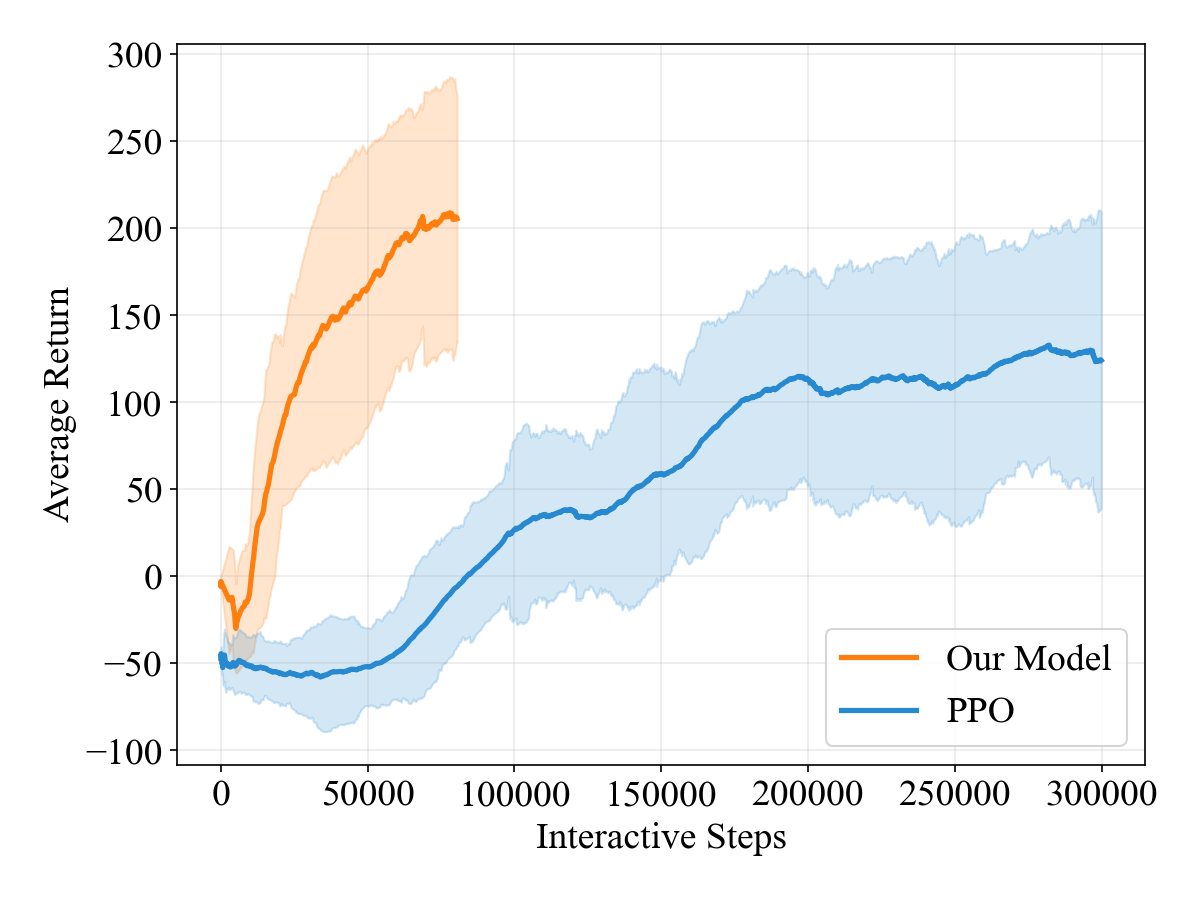
\includegraphics[width=0.9\columnwidth]{figures/train_vs_ppo.png}  
    \caption{A comparison between our model with PPO. The solid lines represent the averaged return, while the shaded area indicates the variability around the mean.} 
    \label{fig:train_return_vs_ppo} 
\end{figure}

\subsection{Ablation Studies}

We conducted a series of ablation experiments, and the results are presented in Figure~\ref{fig:Training curve} and Table~\ref{tab:ablation}. Our ablation study compares four model variants: ImgOnly, a baseline using solely images with reward and continuation heads; Img+Head, which adds lane and neighbor detection heads to image input; and Img+Head+Phys, our full framework integrating both multi-modal inputs and five supervision heads. Table~\ref{tab:ablation} also includes an experiment where the reward and continuation heads were removed.

The result indicate that adding the lane/neighbor heads to the image-only model improved the mean return (MR) by $9.7\%$ and the success rate (SR) by $16$ percentage points. After further incorporating physical information as input, MR continued to improve by $12.2\%$, with a total improvement of $23.1\%$. In addition, the reward and continuation heads played a crucial role in our experiment, and the performance of the model would significantly decline if they were removed.

These results validate that driving-specific supervision and multi-modal inputs are both critical, with their combination yielding synergistic improvements in driving performance.

\begin{figure}[t]
    \centering  
    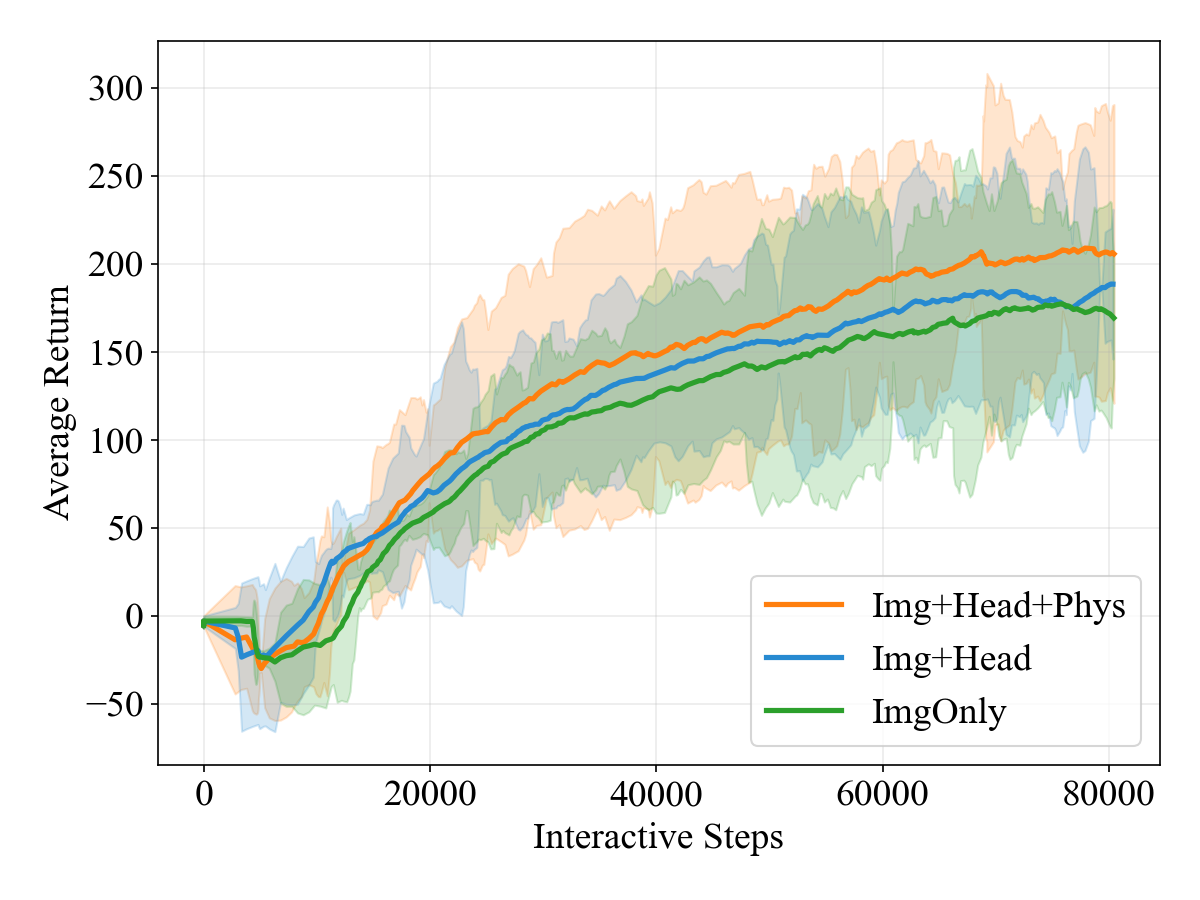
\includegraphics[width=0.9\columnwidth]{figures/compare.png} 
    \caption{Training curves of model variants in the ablation study. ImgOnly (green) uses images input alone; Img+Head (blue) adds lane and neighbor supervision heads; Img+Head+Phys (orange) further incorporates vehicle physics as input.} 
    \label{fig:Training curve} 
\end{figure}


\begin{table}[htbp]
\centering
\caption{Ablation Study Results}
\label{tab:ablation}
\begin{tabular}{@{}>{\bfseries}ccccccc@{}}
\toprule
\rowcolor{white}
\multicolumn{2}{c}{\textbf{Input}} & \multicolumn{3}{c}{\textbf{Heads}} & \multicolumn{2}{c}{\textbf{Metrics}} \\
\cmidrule(lr){1-2} \cmidrule(lr){3-5} \cmidrule(lr){6-7}
Image & Phys & Decoder & Rwd/Cont & Lane/Neigh & MR & SR \\
\midrule
\checkmark & $\times$ & \checkmark & \checkmark & $\times$ & 176.5 & 0.17 \\
\checkmark & $\times$ & \checkmark & \checkmark & \checkmark & 193.6 & 0.33 \\
\checkmark & \checkmark & \checkmark & $\times$ & \checkmark & 172.6 & 0.18 \\
\rowcolor{gray!20}
\checkmark & \checkmark & \checkmark & \checkmark & \checkmark & 217.2 & 0.49 \\
\bottomrule
\end{tabular}
\end{table}
\subsection{Synthetic Scenarios}
\begin{figure*}[t]
    \centering  
    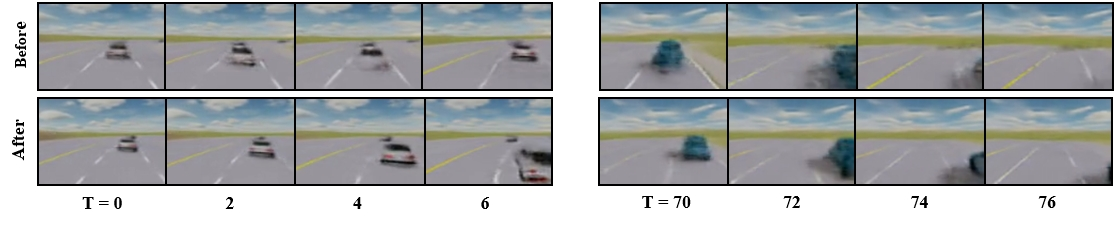
\includegraphics[width=1.0\textwidth]{figures/imagine_compare.png}  
    \caption{Comparison of imagination quality across model variants. Top row: ImgOnly generates physically inconsistent rollouts with blurred vehicle positions (left) and confused lane markings (right). Bottom row: Img+Head+Phys produces stable, physically plausible predictions with correct semantic preservation of surrounding vehicles and lane markings.} 
    \label{fig:Imagined World} 
\end{figure*}
We compare the imagination quality of different model variants. As illustrated in Figure~\ref{fig:Imagined World}, the world model trained with only image input (ImgOnly) generates physically inconsistent rollouts. For example, when the ego car is preparing to overtake, the position of the preceding vehicle becomes blurred and undergoes abrupt, unrealistic shifts. In lane-changing scenarios, the model frequently confuses yellow solid lines with white dashed lines. In contrast, the combination of vehicle kinematics and auxiliary supervision effectively alleviates these problems. The imagined trajectories now maintain stable and physically plausible states for surrounding vehicles during interactions, and correctly preserve the color and type of lane markings during maneuvers, demonstrating improved physical grounding and semantic consistency in the latent space.

\iffalse
\subsection{Mask Experiment}
Before designing the framework, we conducted masking experiments to identify key driving information using a 31-dimensional observation vector comprising lane border distances (2D), heading angle (1D), vehicle physics (5D), lane center offset (1D), navigation (10D), and neighboring vehicle information (12D).

The Influence is calculated as (Baseline Return - Masked Return) / Baseline Return, quantifying the performance drop when a specific information group is removed.

The results in Table~\ref{tab:mask experiment} reveal that lane border distance and heading angle are most critical for lane keeping, motivating our Lane Detection Head design. A performance drop of 25-30\% is also observed when physics and neighbor information are masked, justifying their inclusion for dynamic control and collision avoidance. Notably, the 31D vector alone achieves strong performance, confirming that high-level semantics suffice for the task and guiding our approach to explicitly encode these structures in the world model.

\begin{table}[htbp]
\centering
\caption{Mask Experiment}
\label{tab:mask experiment}
\begin{tabular}{@{}lcccc@{}}
\toprule
\textbf{Group} & \textbf{Dim} & \textbf{Mean Return} & \textbf{Top Reason} & \textbf{Influence} \\
\midrule
Baseline & 31 & 208.1 ($\pm$73.4) & -- & -- \\
Border & 2 & 48.6 ($\pm$27.4) & Out of Road & 76.6\% \\
Heading & 1 & 91.8 ($\pm$81.5) & Out of Road & 55.9\% \\
Phys & 5 & 149.5 ($\pm$6.4) & Out of Road & 28.1\% \\
Center & 1 & 147.8 ($\pm$52.1) & Collision with Vehicle & 28.9\% \\
Nav & 10 & 151.1 ($\pm$10.1) & Out of Road & 27.4\% \\
Neigh & 12 & 156.5 ($\pm$35.6) & Collision with Vehicle & 24.7\% \\
\bottomrule
\end{tabular}
\end{table}
\fi


